\documentclass[fleqn,12pt,a4paper]{olplainarticle}
% Use option lineno for line numbers 

\usepackage{hyperref}

\title{DUNE Timing System (DTS) Safety Engineering Design Review (SEDR) Documentation for GPS Interface Board (GIB)}

\author[1]{D. Antic}
\author[1]{D. Cussans}
\author[2]{J. Sensenig}
\author[1]{S. Trilov}
\affil[1]{H.H. Wills Physics Laboratory, Bristol, UK}
\affil[2]{David Rittenhouse Laboratory, Philadelphia, USA}

\begin{document}


%\keywords{Keyword1, Keyword2, Keyword3}

\begin{abstract}
This document provides information needed for a review of the electrical safety of the DUNE Timing System(DTS) GPS Interface Board (GIB). An overview of the DTS hardware is given in EDMS document EDMS-XXXXX and should be read in conjunction with this document.
\end{abstract}


\flushbottom

\maketitle

\thispagestyle{empty}

\section{Introduction}

The DUNE Timing System has hardware components both above ground and below ground. At the far detector the above ground hardware will be at the SURF Ross and Yates areas and the below ground in the DAQ cabins above each far detector cryostat. At the near detector the above ground hardware will be at Fermilab in a location accessible to the ACLK,TCLK and BSCLK accelerator signals with the below ground hardware in the near detector hall.

The above ground hardware at each of the Ross and Yates areas consists of a COTS GPS disciplined oscillator with associated antenna, lightning protection etc. providing timing information to a custom GPS Interface Board (GIB). The below ground hardware in each of the far detector caverns consists of a COTS MicroTCA crate housing COTS PSUs, MCH, JSM and fan-trays along with a custom MicroTCA Inteface Board (MIB) and multiple semi-custom FPGA based AFC boards hosting custom Fibre Interface Boards (FIBs). Each far detector cavern will have two MicroTCA crates.
Figure \ref{fig:dts_fd_block_diagram} illustrates the location of DTS hardware at the far detector.

\begin{figure}[ht]
\centering
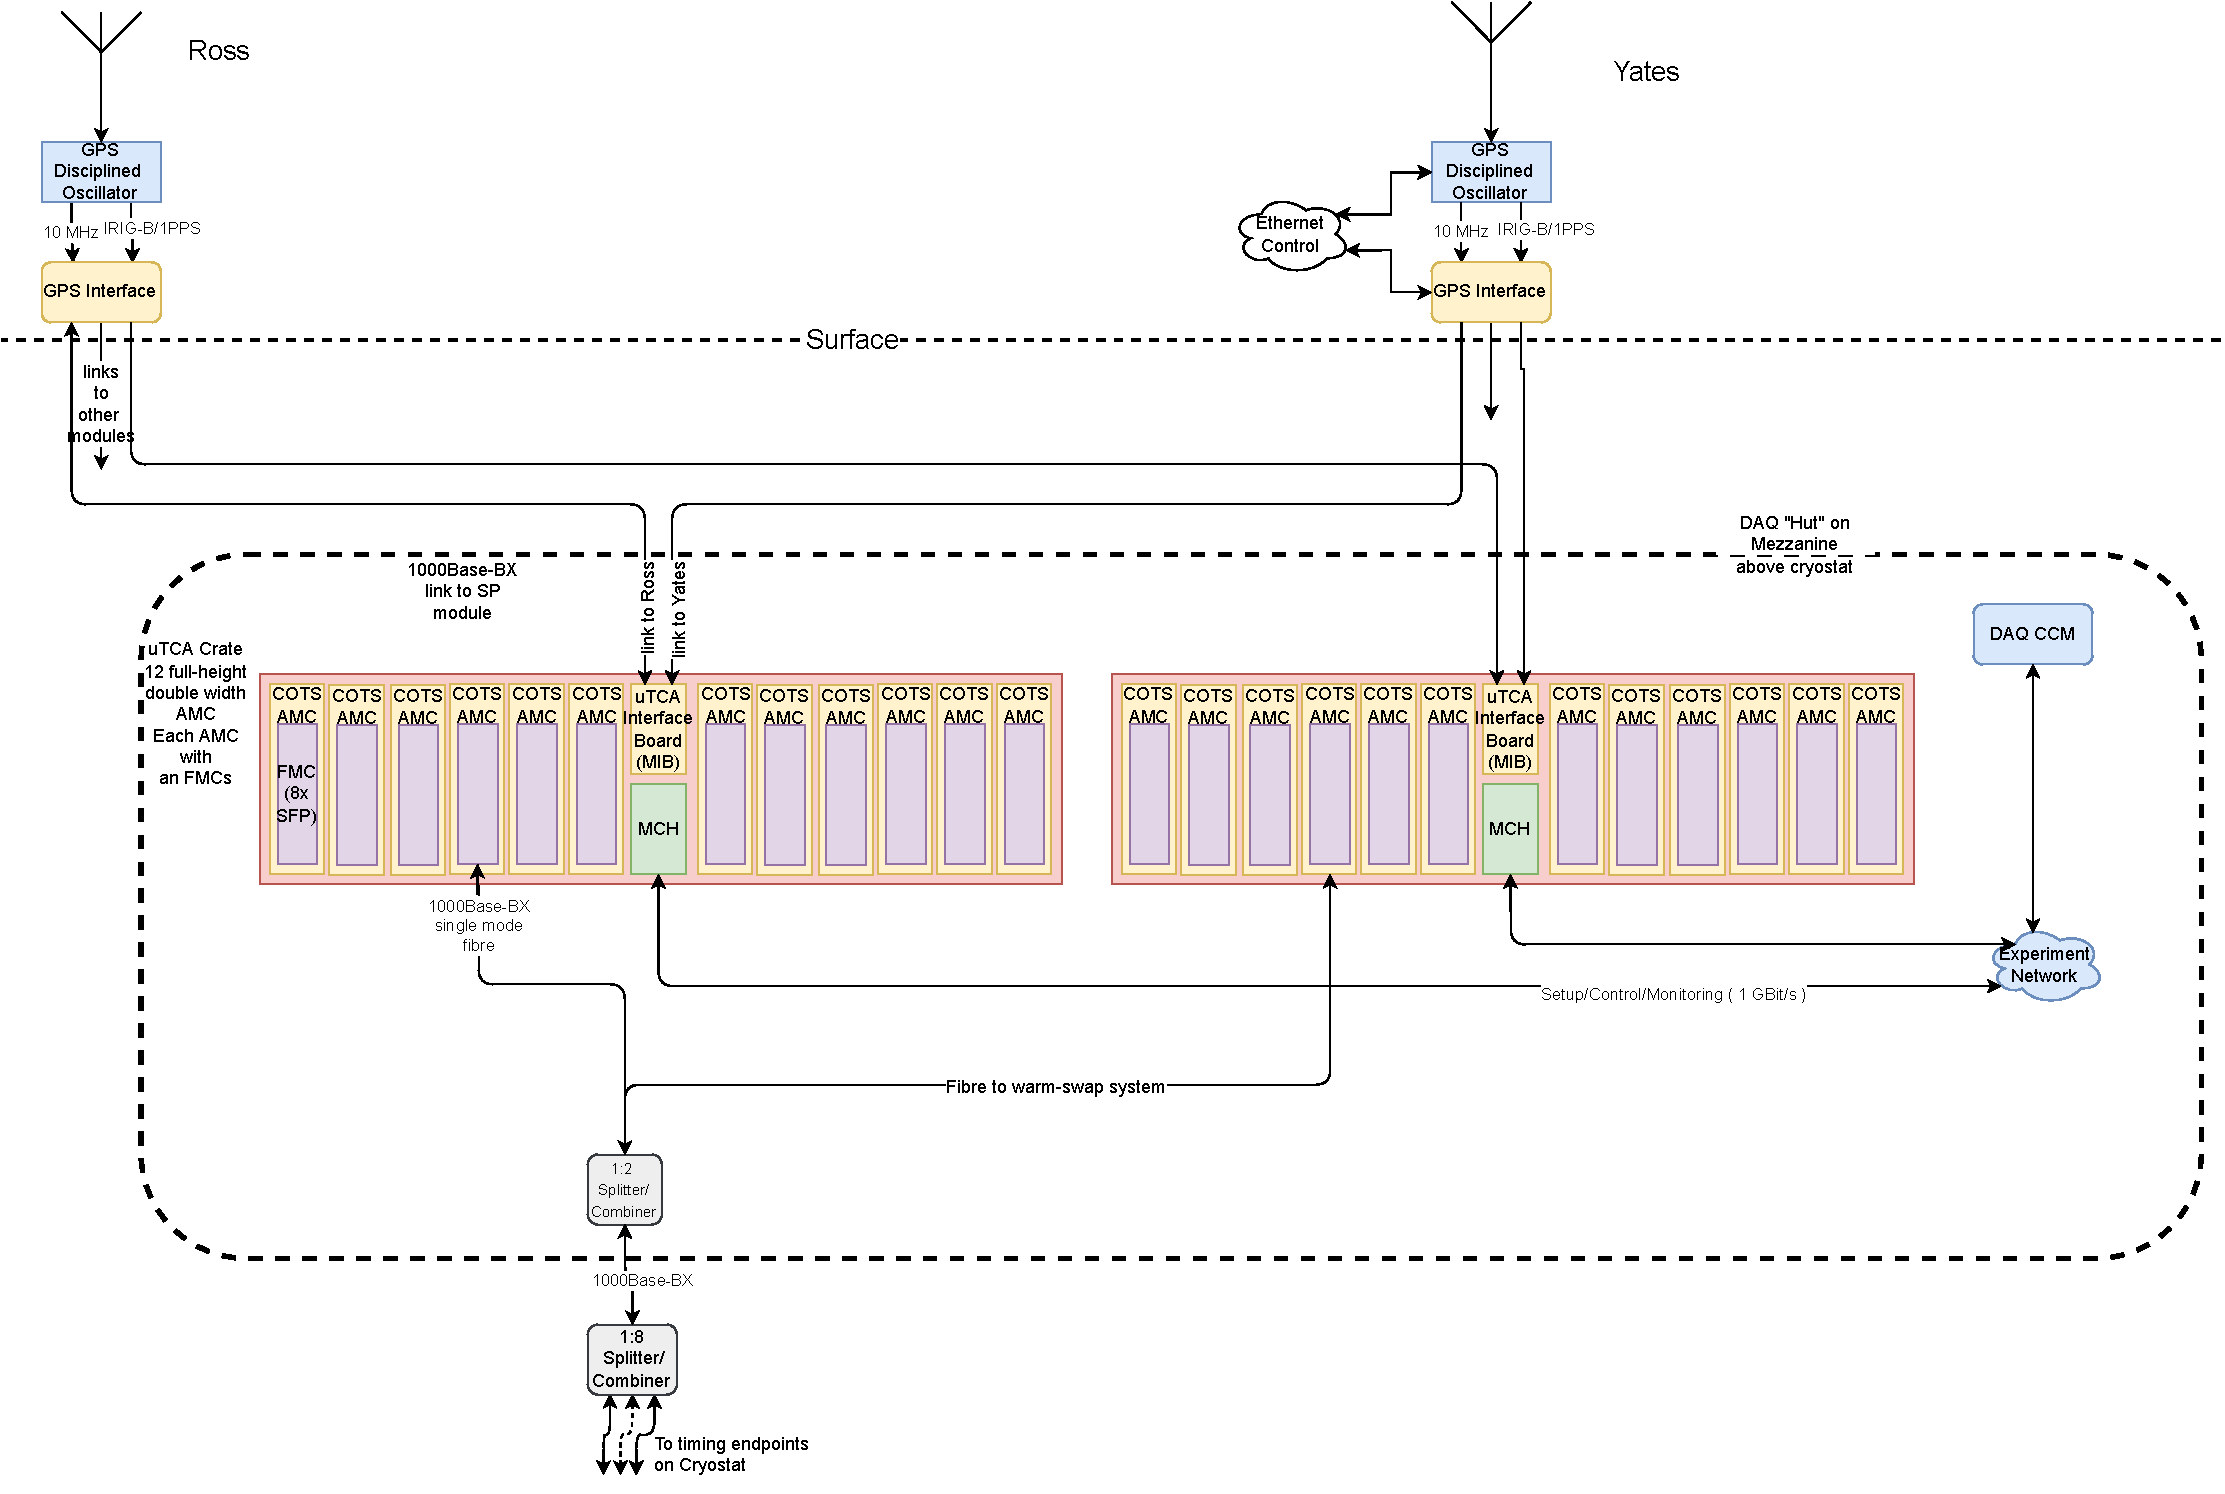
\includegraphics[width=\linewidth]{dune_timing_system_block_diagram_twepp22_1sept22_02.drawio.pdf}
\caption{Block Diagram of DUNE Far Detector Timing Hardware.}
\label{fig:dts_fd_block_diagram}
\end{figure}

\section{Above Ground Hardware}

\subsection{GPS Disciplined Oscillator}

The GPS Disciplined Oscillator (GPS-DO) for the DTS is the \href{https://safran-navigation-timing.com/product/securesync-time-and-frequency-reference-system}{SecureSync Time Server} with IRIG output option fitted.

\subsection{GPS Interface Board}

The GIB is coupled to a COTS FPGA module (Enclustra \href{https://www.enclustra.com/en/products/fpga-modules/mars-ax3/}{AX3}/\href{https://www.enclustra.com/en/products/base-boards/mars-pm3/}{PM3} combination) and mounted in a custom 19-inch rack mounting enclosure. Power is provided at 12V from an external COTS AC-DC power supply. Figure \ref{fig:dts_gib_power_block_diagram} illustrates the powering arrangements for the GIB. It is anticipated that, in addition to over-current protection provided by fuses, temperature control and monitoring will be provided an slow control microcontroller with an  ``Ethercat'' interface. If no active slow control is possible an over-temperature fuse will be used. Figure \ref{fig:dts_gibV1_photo} shows the current GIB prototype.

\begin{figure}[ht]
\centering
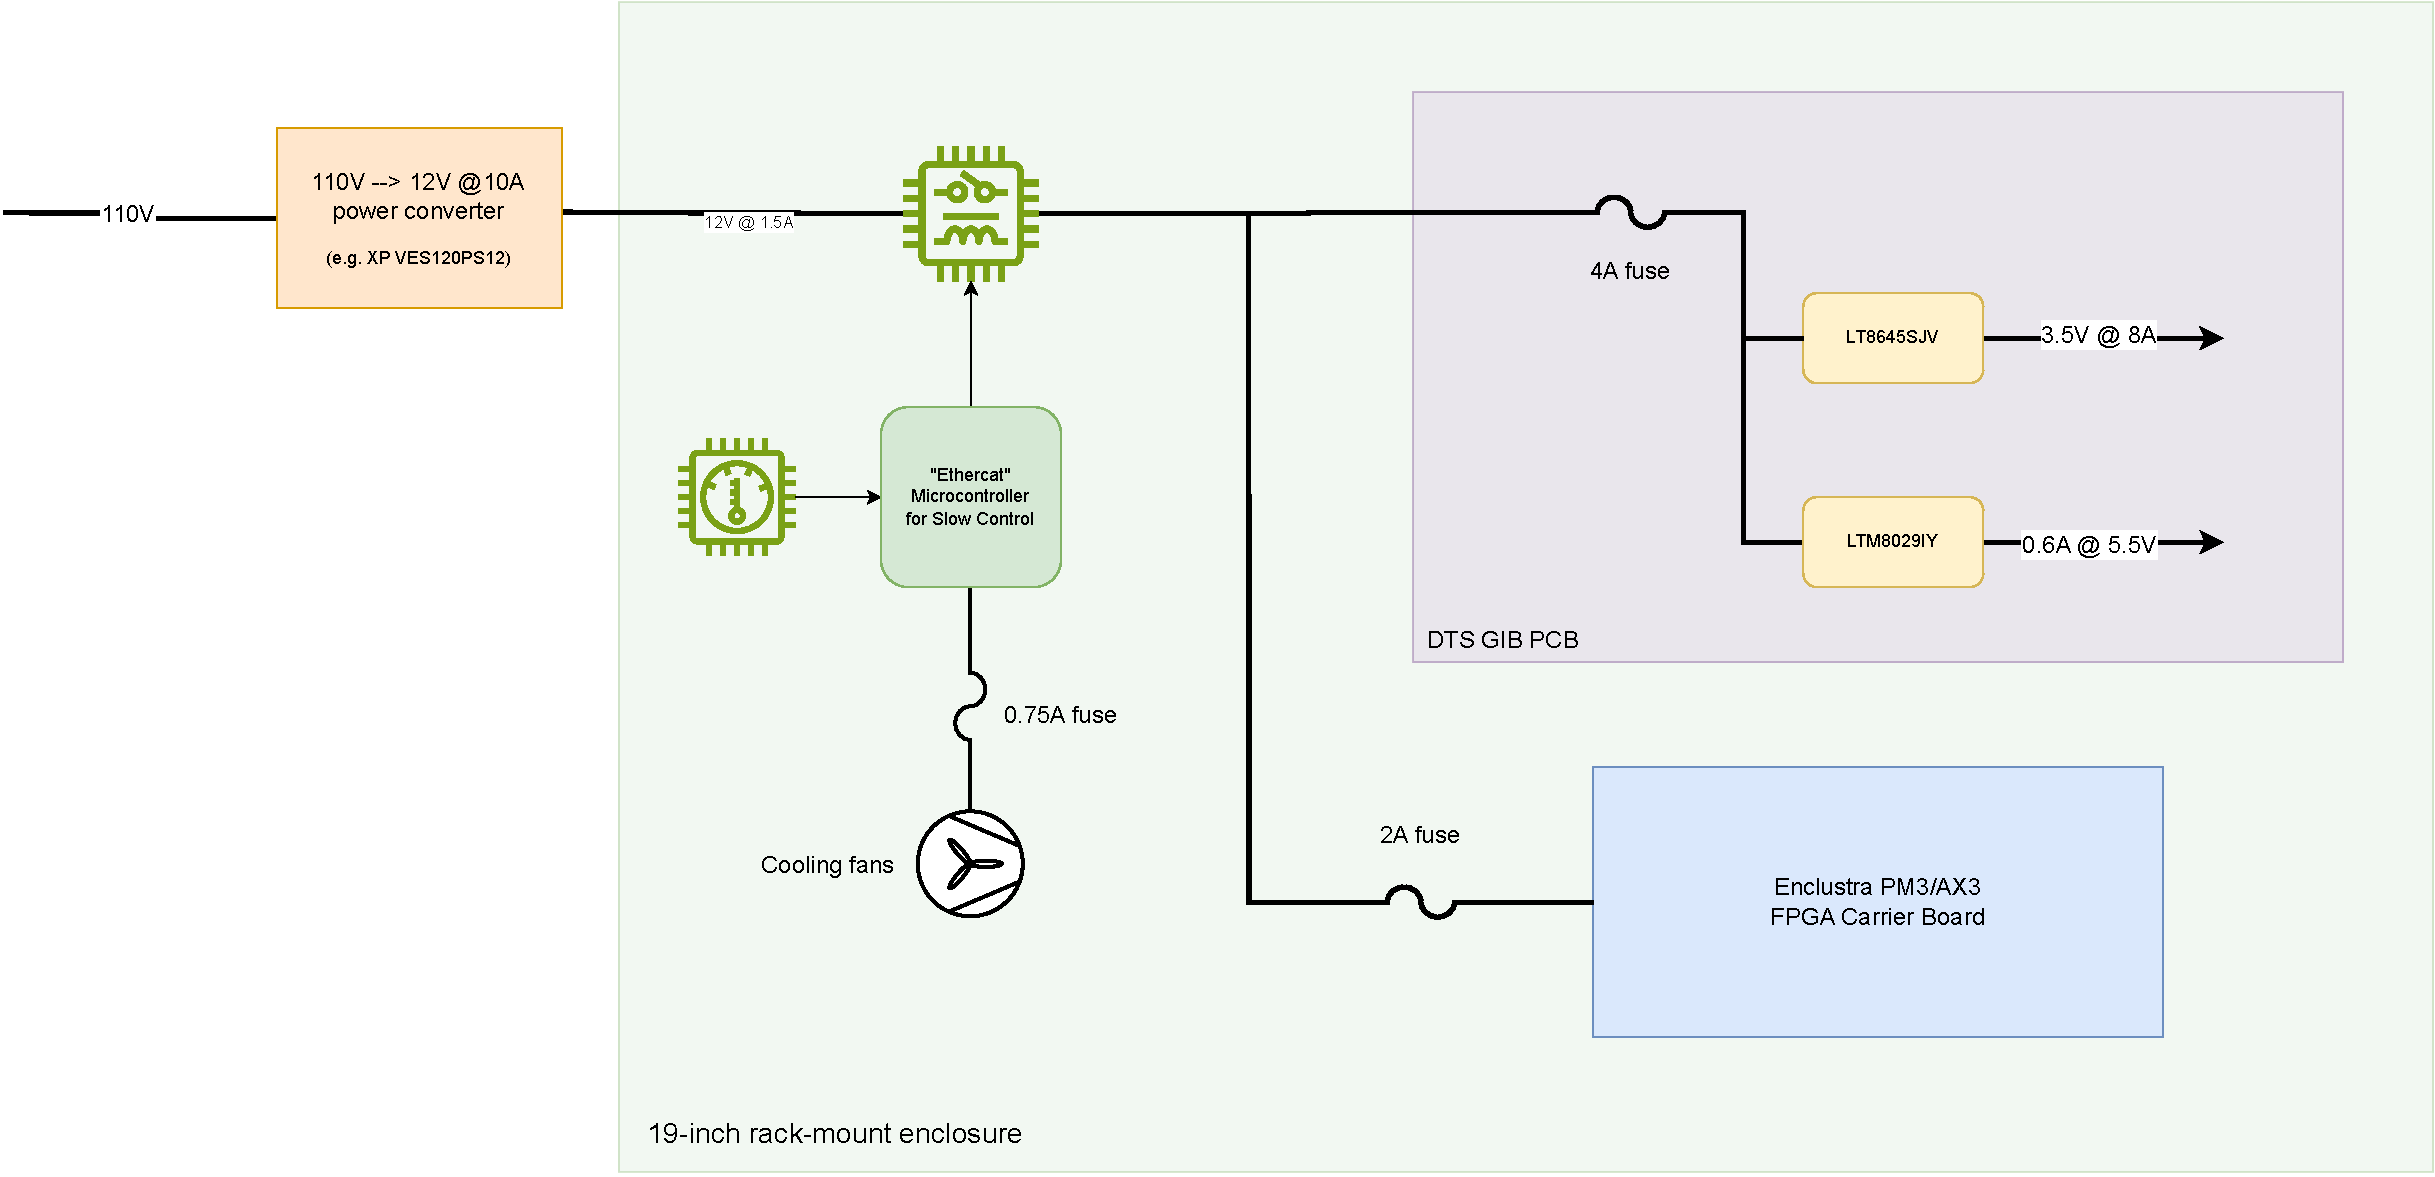
\includegraphics[width=\linewidth]{dts_gib_power_block_diagram_v1-231219.drawio.pdf}
\caption{Block diagram of powering arrangements for GIB}
\label{fig:dts_gib_power_block_diagram}
\end{figure}

\begin{figure}[ht]
\centering
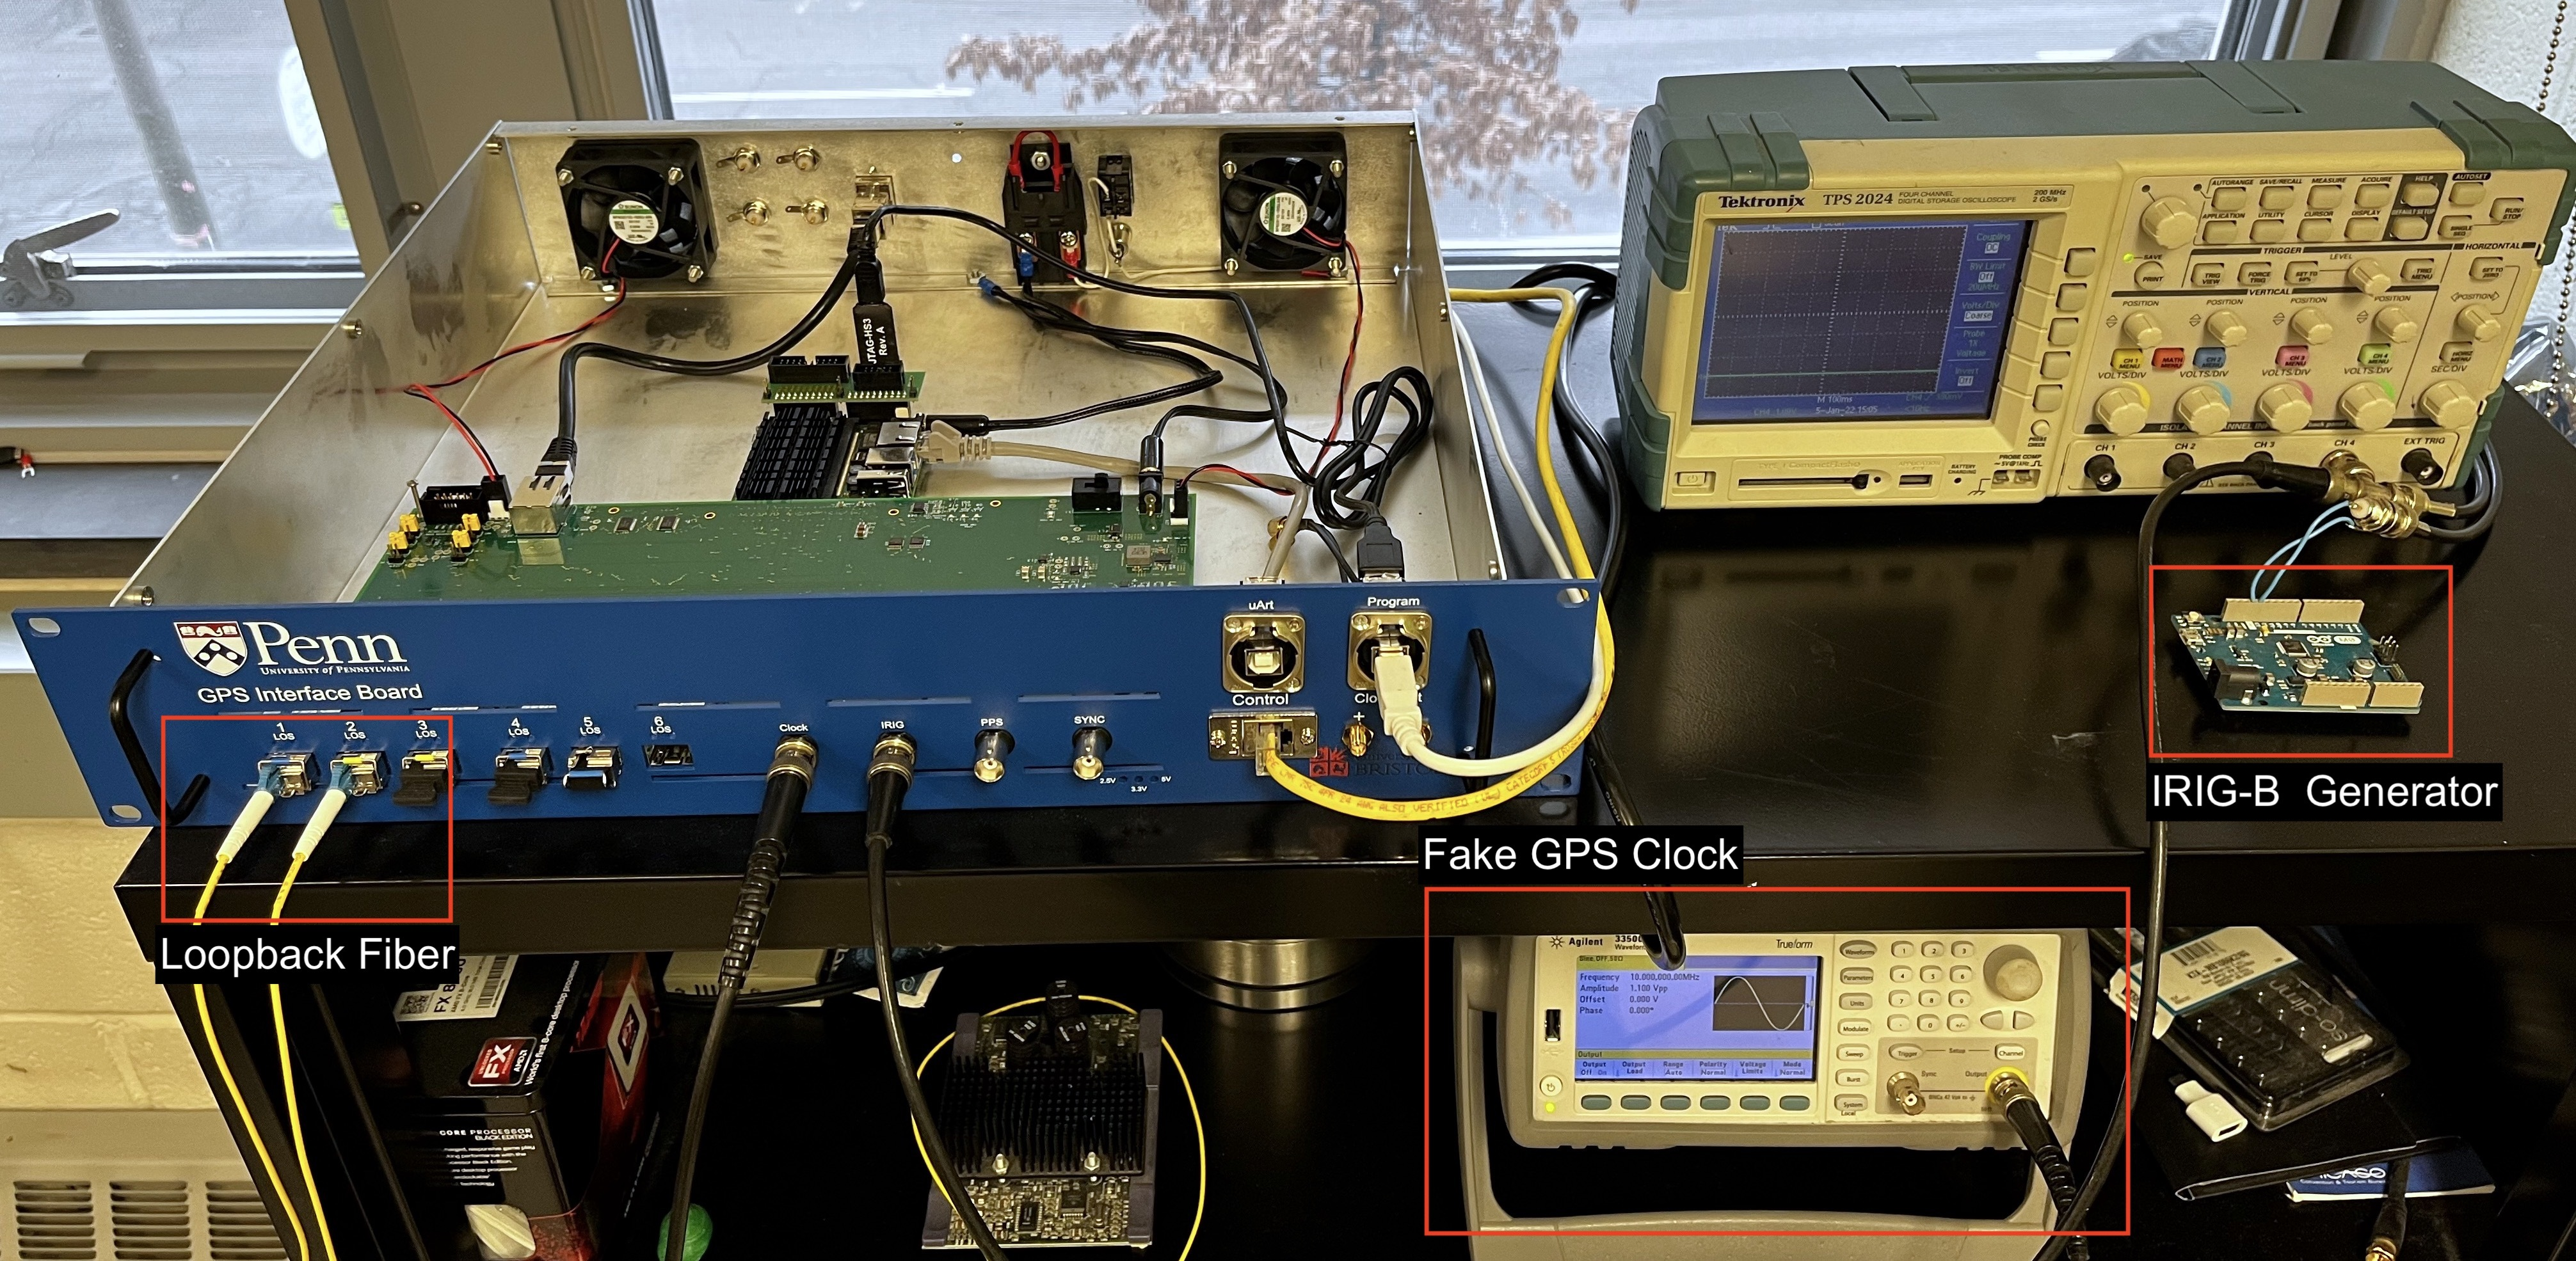
\includegraphics[width=0.85\linewidth]{gib_teststand_setup_annotated.JPG}
\caption{Photograph of current GIB prototype}
\label{fig:dts_gibV1_photo}
\end{figure}

\section{Below Ground Hardware}

All DTS hardware will be in 19-inch racks with front-to-back cooling located in the DAQ areas above the cryostats. Figure \ref{fig:dts_crate_block_diagram} illustrates the arrangement of DTS hardware in a rack. Figures \ref{fig:dts-utca-front-view} and \ref{fig:dts-utca-rear-view} illustrate the front and rear of a DTS MicroTCA crate. Figure \ref{fig:dts-utca-test-system-photo} is a photograph of the MicroTCA system used for DTS hardware development.

\begin{figure}[ht]
\centering
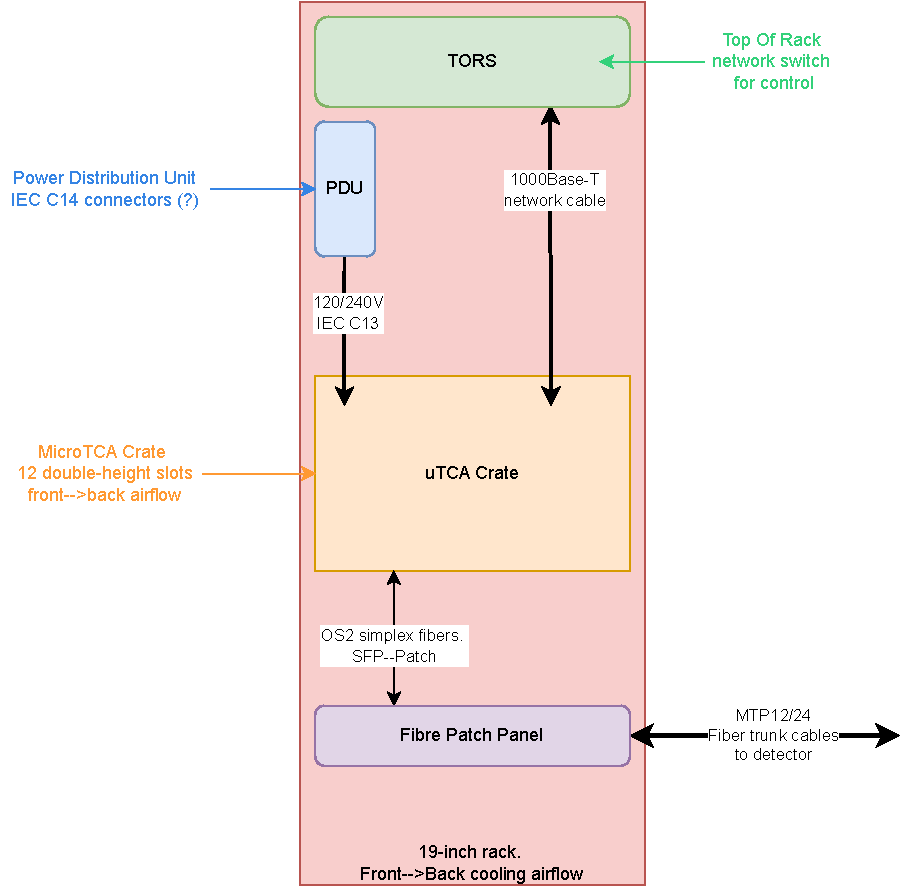
\includegraphics[width=0.7\linewidth]{dts_overall_rack-v1-231215.drawio.pdf}
\caption{Arrangement of DTS hardware in a DAQ RACK.}
\label{fig:dts_crate_block_diagram}
\end{figure}

\begin{figure}
  \centering
  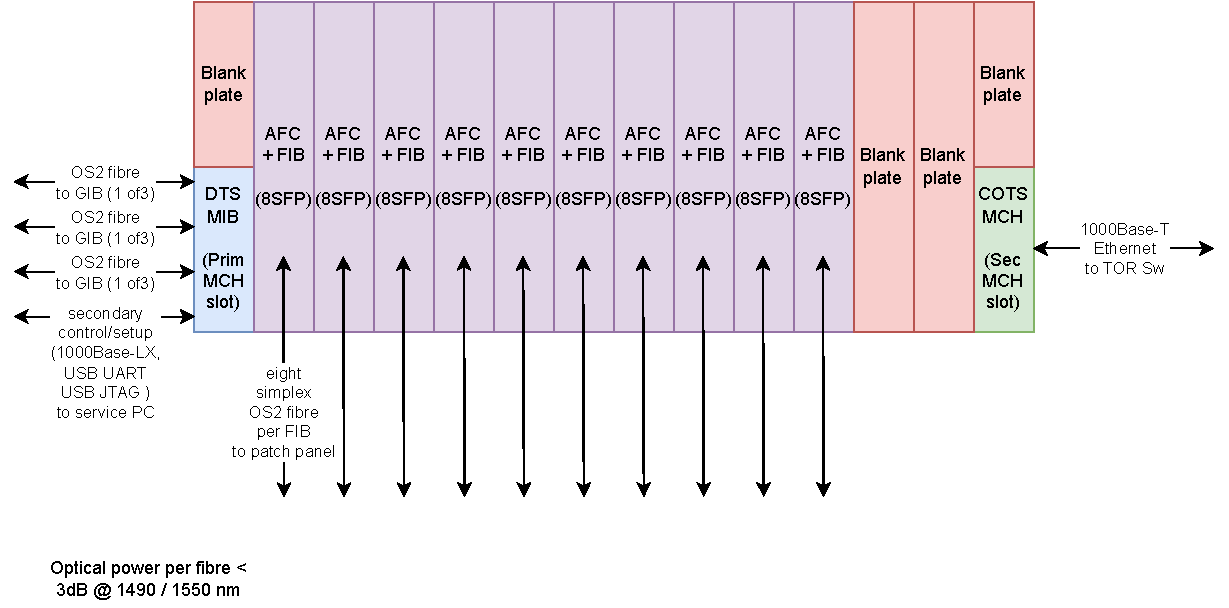
\includegraphics[width=\linewidth]{dts_utca_crate-front-v1-231215.drawio.pdf}
  \caption{Diagram showing front view of DTS uTCA crate.}
  \label{fig:dts-utca-front-view}
\end{figure}

\begin{figure}
  \centering
  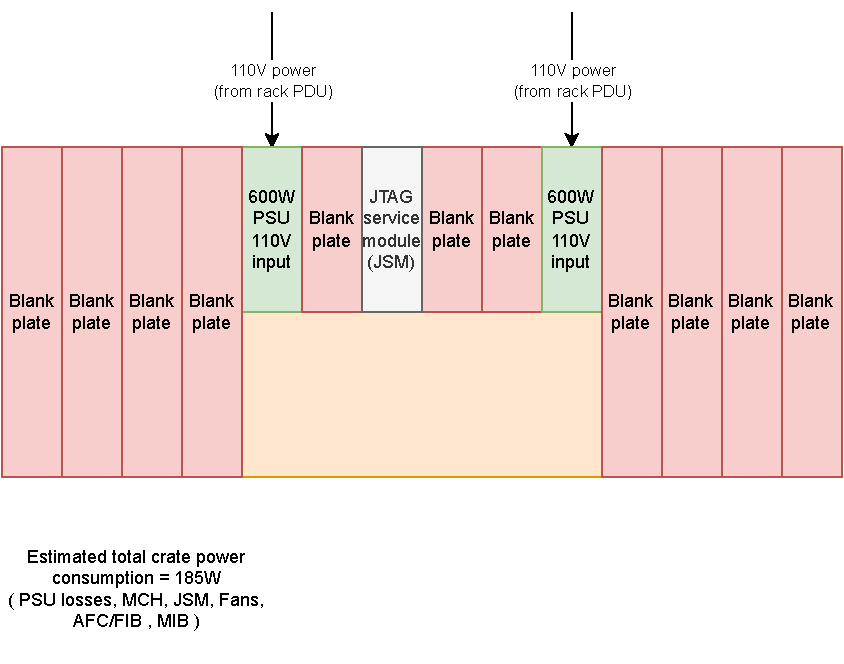
\includegraphics[width=0.8\linewidth]{dts_utca_crate-rear-v1-231215.drawio.pdf}
  \caption{Diagram showing rear view of DTS uTCA crate.}
  \label{fig:dts-utca-rear-view}
\end{figure}

\begin{figure}
  \centering
  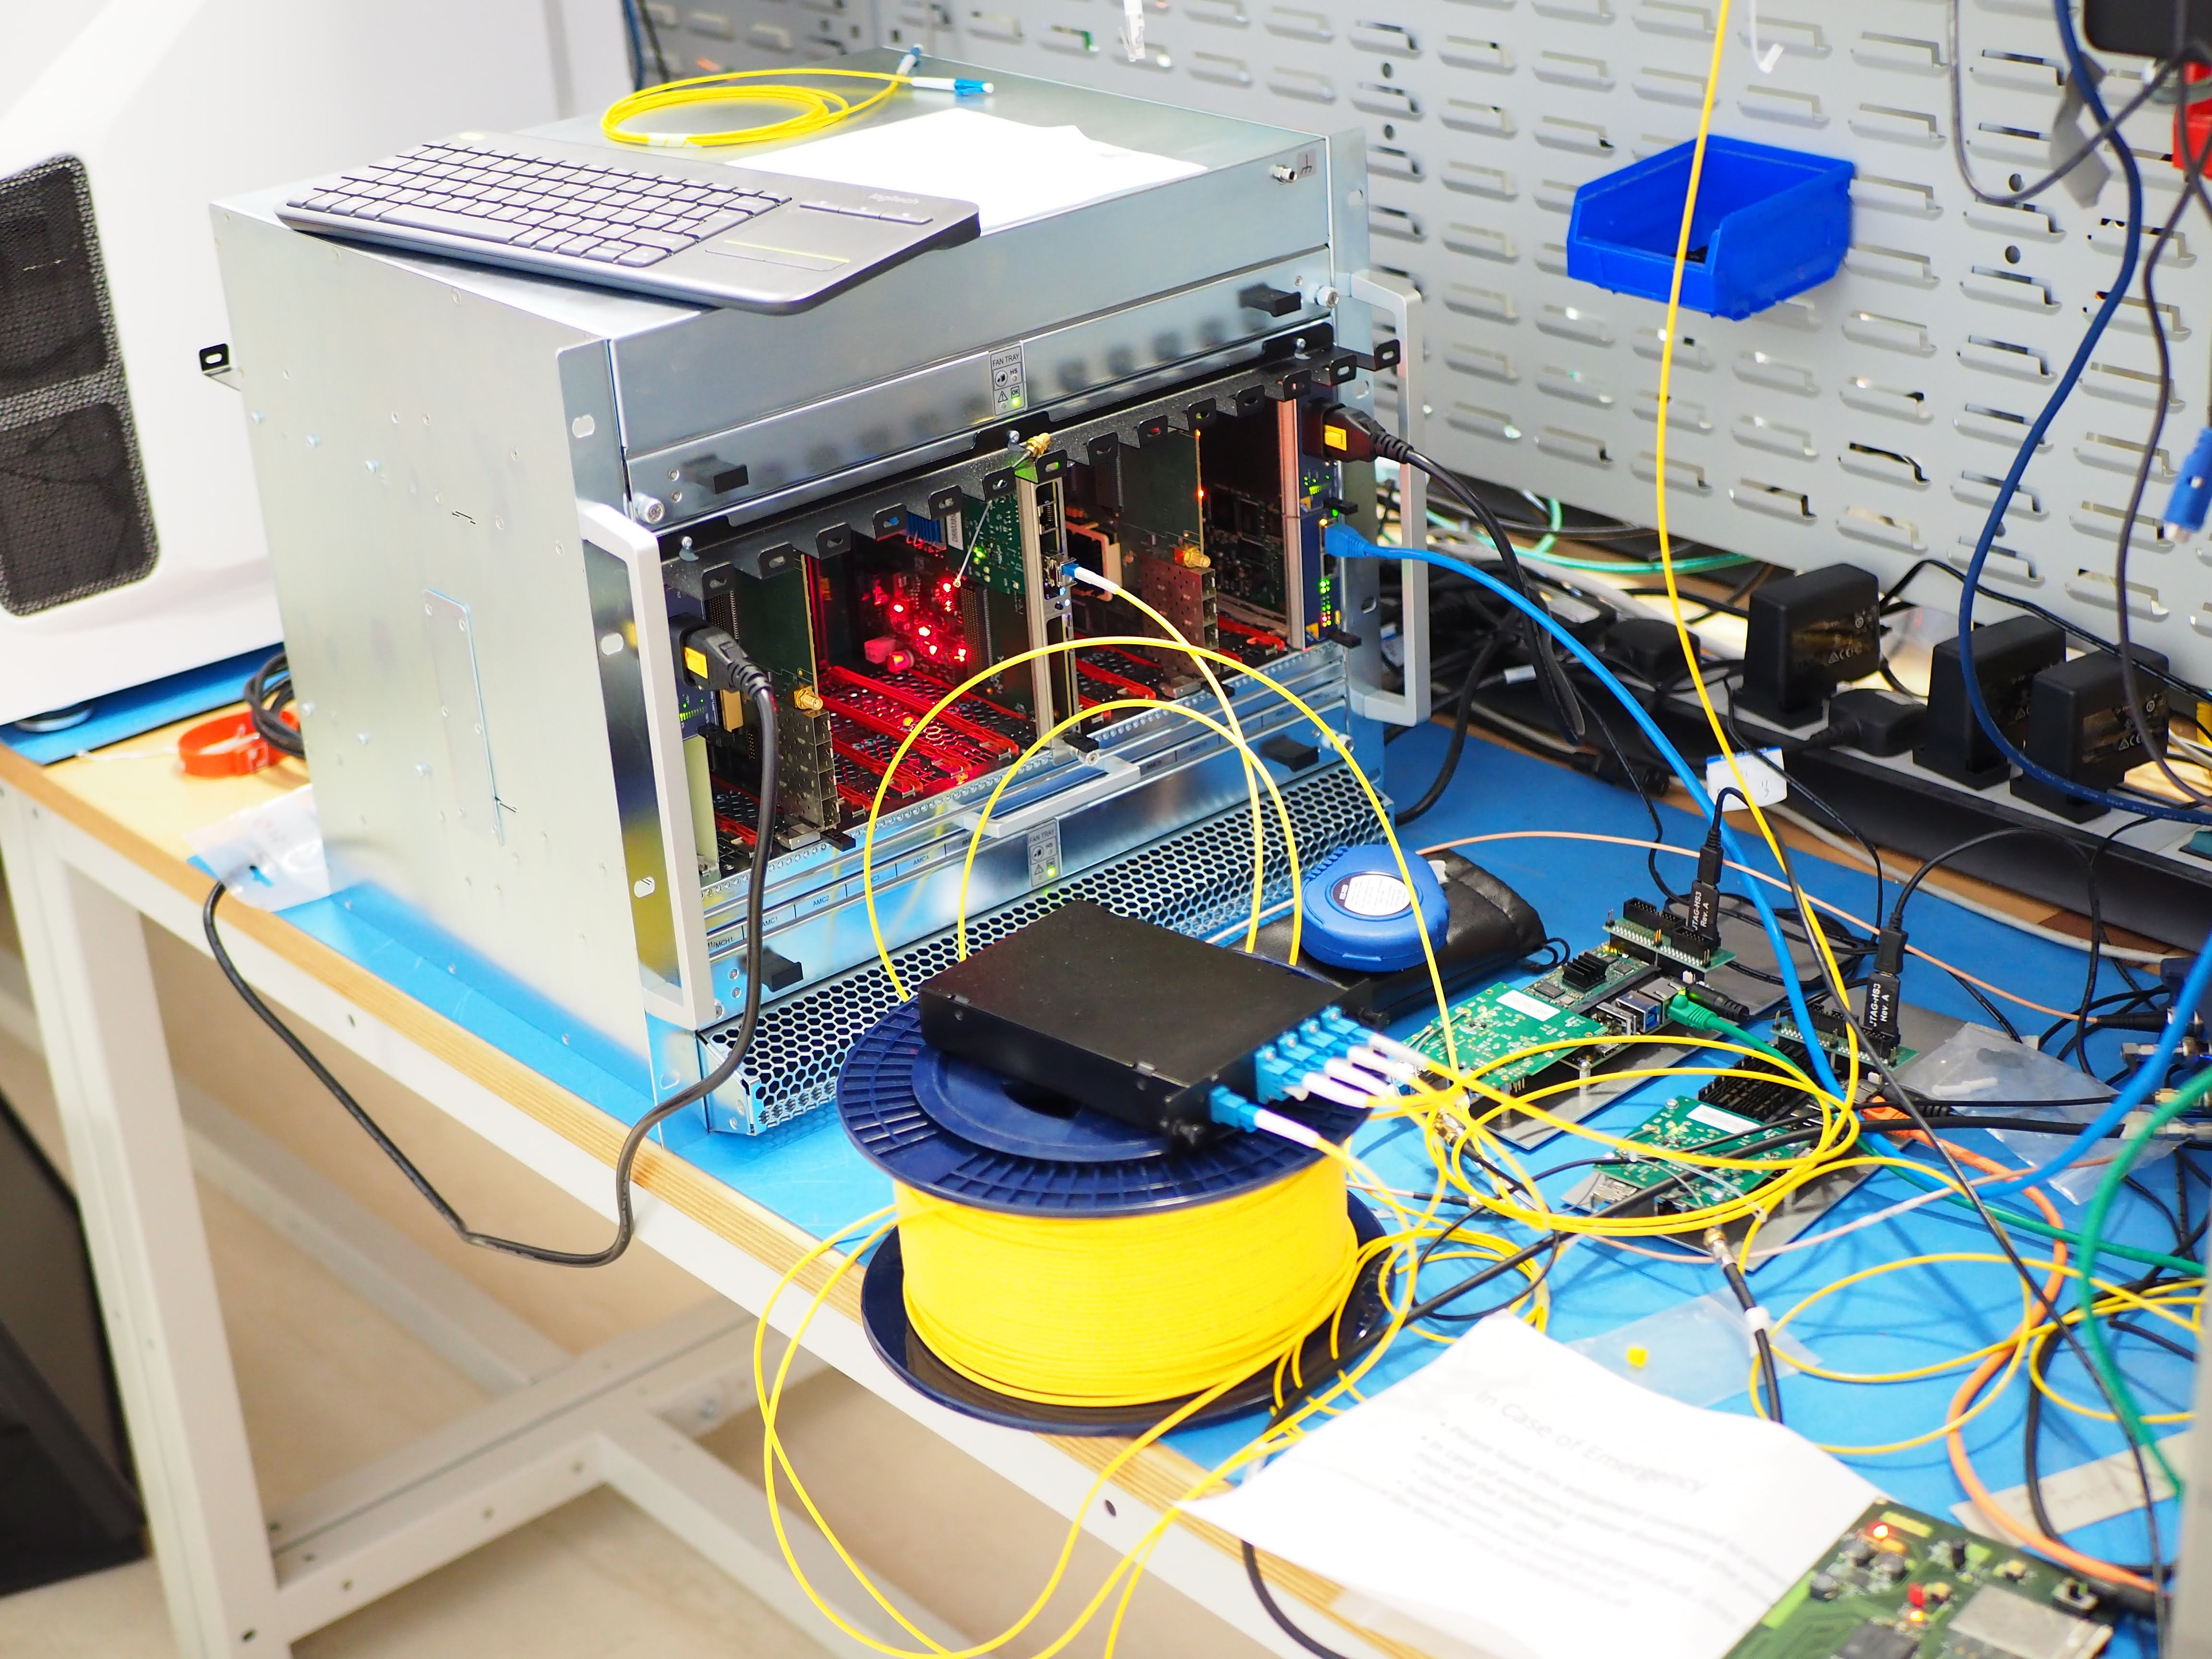
\includegraphics[width=0.8\linewidth]{P7150030.JPG}
  \caption{Photograph of MicroTCA test system.}
  \label{fig:dts-utca-test-system-photo}
\end{figure}


\subsection{MicroTCA Crate}

The MicroTCA crate is a Schroff/nVent model \href{https://schroff.nvent.com/en-gb/products/enc11890-170}{11890170} unit with front-to-back cooling, 12 double-height,double-width slots and two redundant fan-trays 

\subsection{COTS MicroTCA Modules}

\begin{itemize}
    \item {\bf Power Supply Module}   \href{https://nateurope.com/product/nat-pm-ac600-600w-ac-power-module-mtca0/}{NAT-PM-AC600}. Two per crate in redundant configuration.
    \item {\bf MicroTCA Carrier Hub} \href{https://nateurope.com/product/nat-mch/}{NAT-MCH}. Provides a setup, control and monitoring link over 1GBit/s Ethernet.
    \item {\bf JTAG Service Module} \href{https://nateurope.com/product/nat-jsm/}{NAT-JSM}. Used for in-situ firmware updates.
\end{itemize}

\subsection{Custom/Semi-Custom MicroTCA Modules}

Each DTS MicroTCA crate has a single MIB and up to twelve semi-custom AFC boards. Each AFC board has a FIB mounted on it.

\subsubsection{MIB}

Timing signals carried on fibres from the GIBs are received at the underground MicroTCA crates by the MicroTCA Interface Board. The MIB has the same form-factor as an MCH with a tongue-2 connector carrying clock and timing data. There is a MIB located in the primary MCH slot of each MicroTCA crate. Figure \ref{fig:dts-mib-powering} illustrates the powering circuitry of the MIB. MicroTCA boards do not usually have fuses since over-current protection is handled by negotiation between the board module management controller (MMC) and the MicroTCA power supply to set a suitable current limit. However, in order to avoid the effort needed to fully qualify our MMC firmware we have added fuses to the MIB as a secondary over-current protection mechanism. Figure \ref{fig:dts-mib-photo} shows a photograph of a prototype MIB.

\begin{figure}
  \centering
  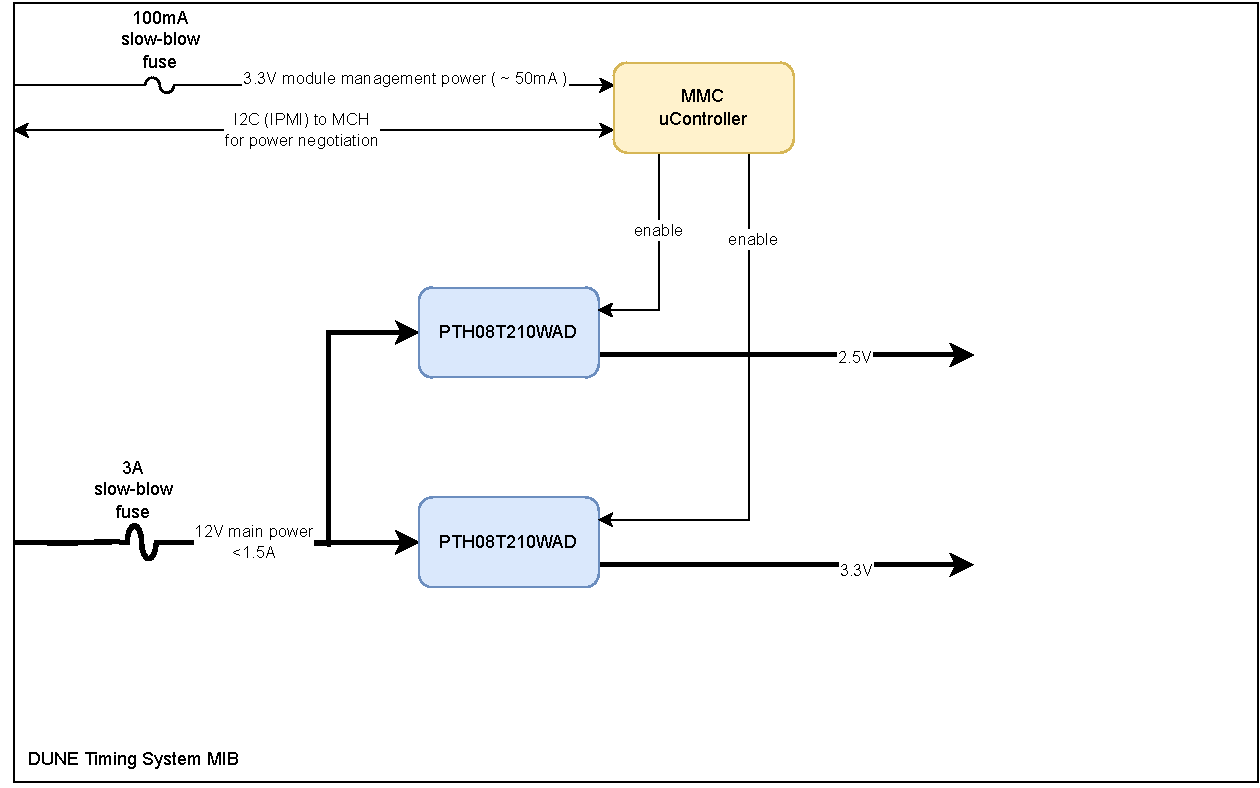
\includegraphics[width=\linewidth]{dts_mib_power_block_diagram_v1-231215.drawio.pdf}
  \caption{Block diagram showing powering of MIB}
  \label{fig:dts-mib-powering}
\end{figure}

\begin{figure}
  \centering
  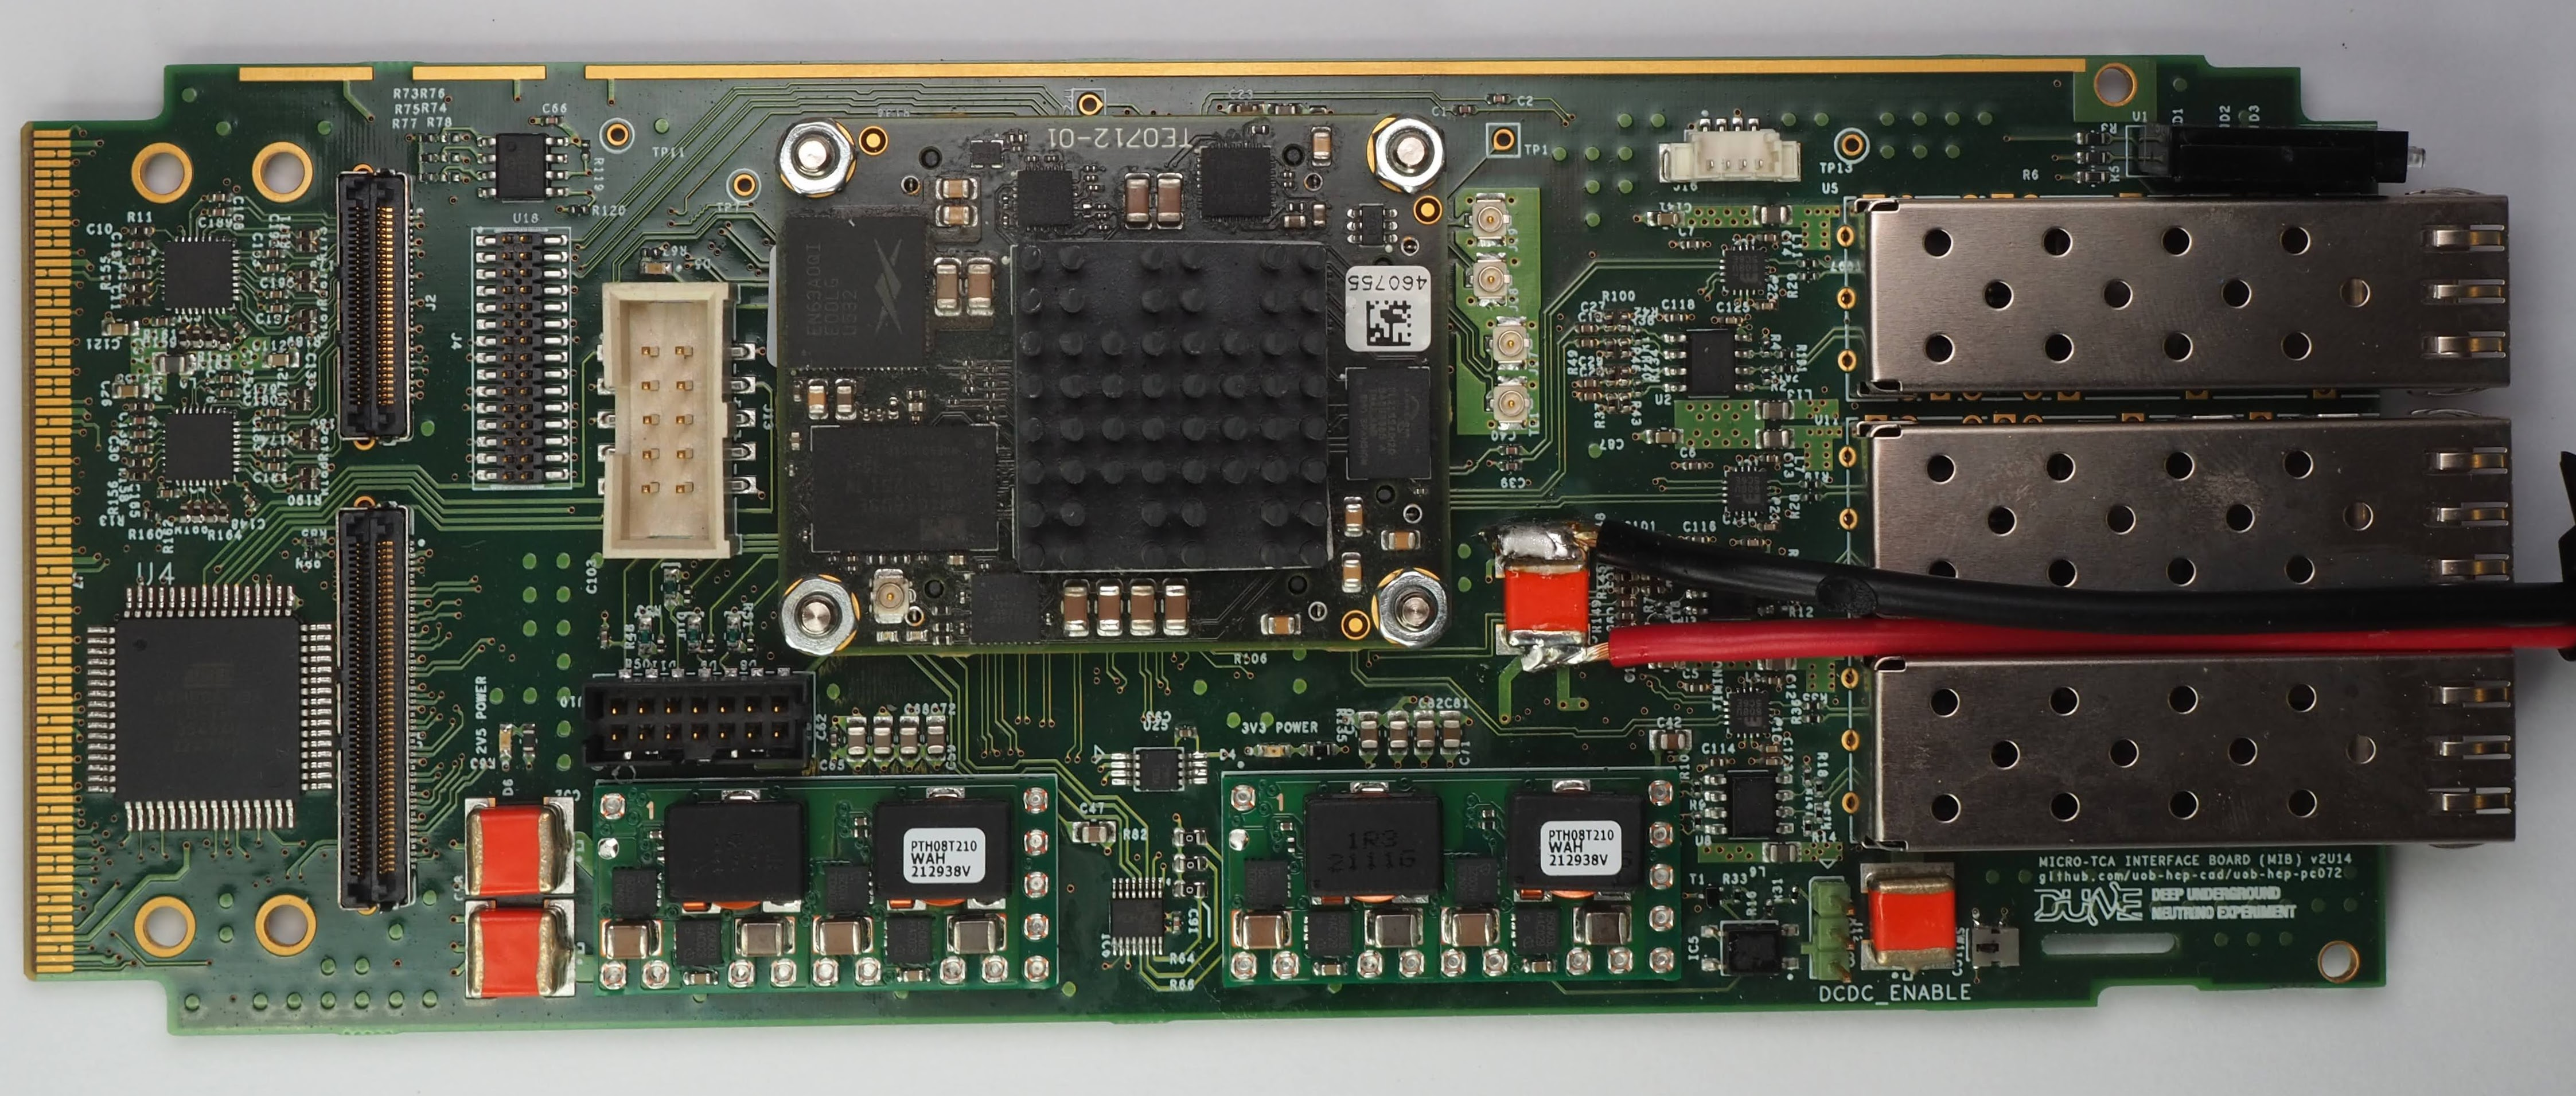
\includegraphics[width=\linewidth]{mib_photo_P8180060.JPG}
  \caption{Photograph of MIB v2}
  \label{fig:dts-mib-photo}
\end{figure}

\subsubsection{FIB}

The fibre interface board is a double width FMC format board with eight SFP sockets mounted on it. It draws its power from the AFC it is mounted on. Figure \ref{fig:dts-fib-photo} shows a prototype FIB.

\begin{figure}
  \centering
  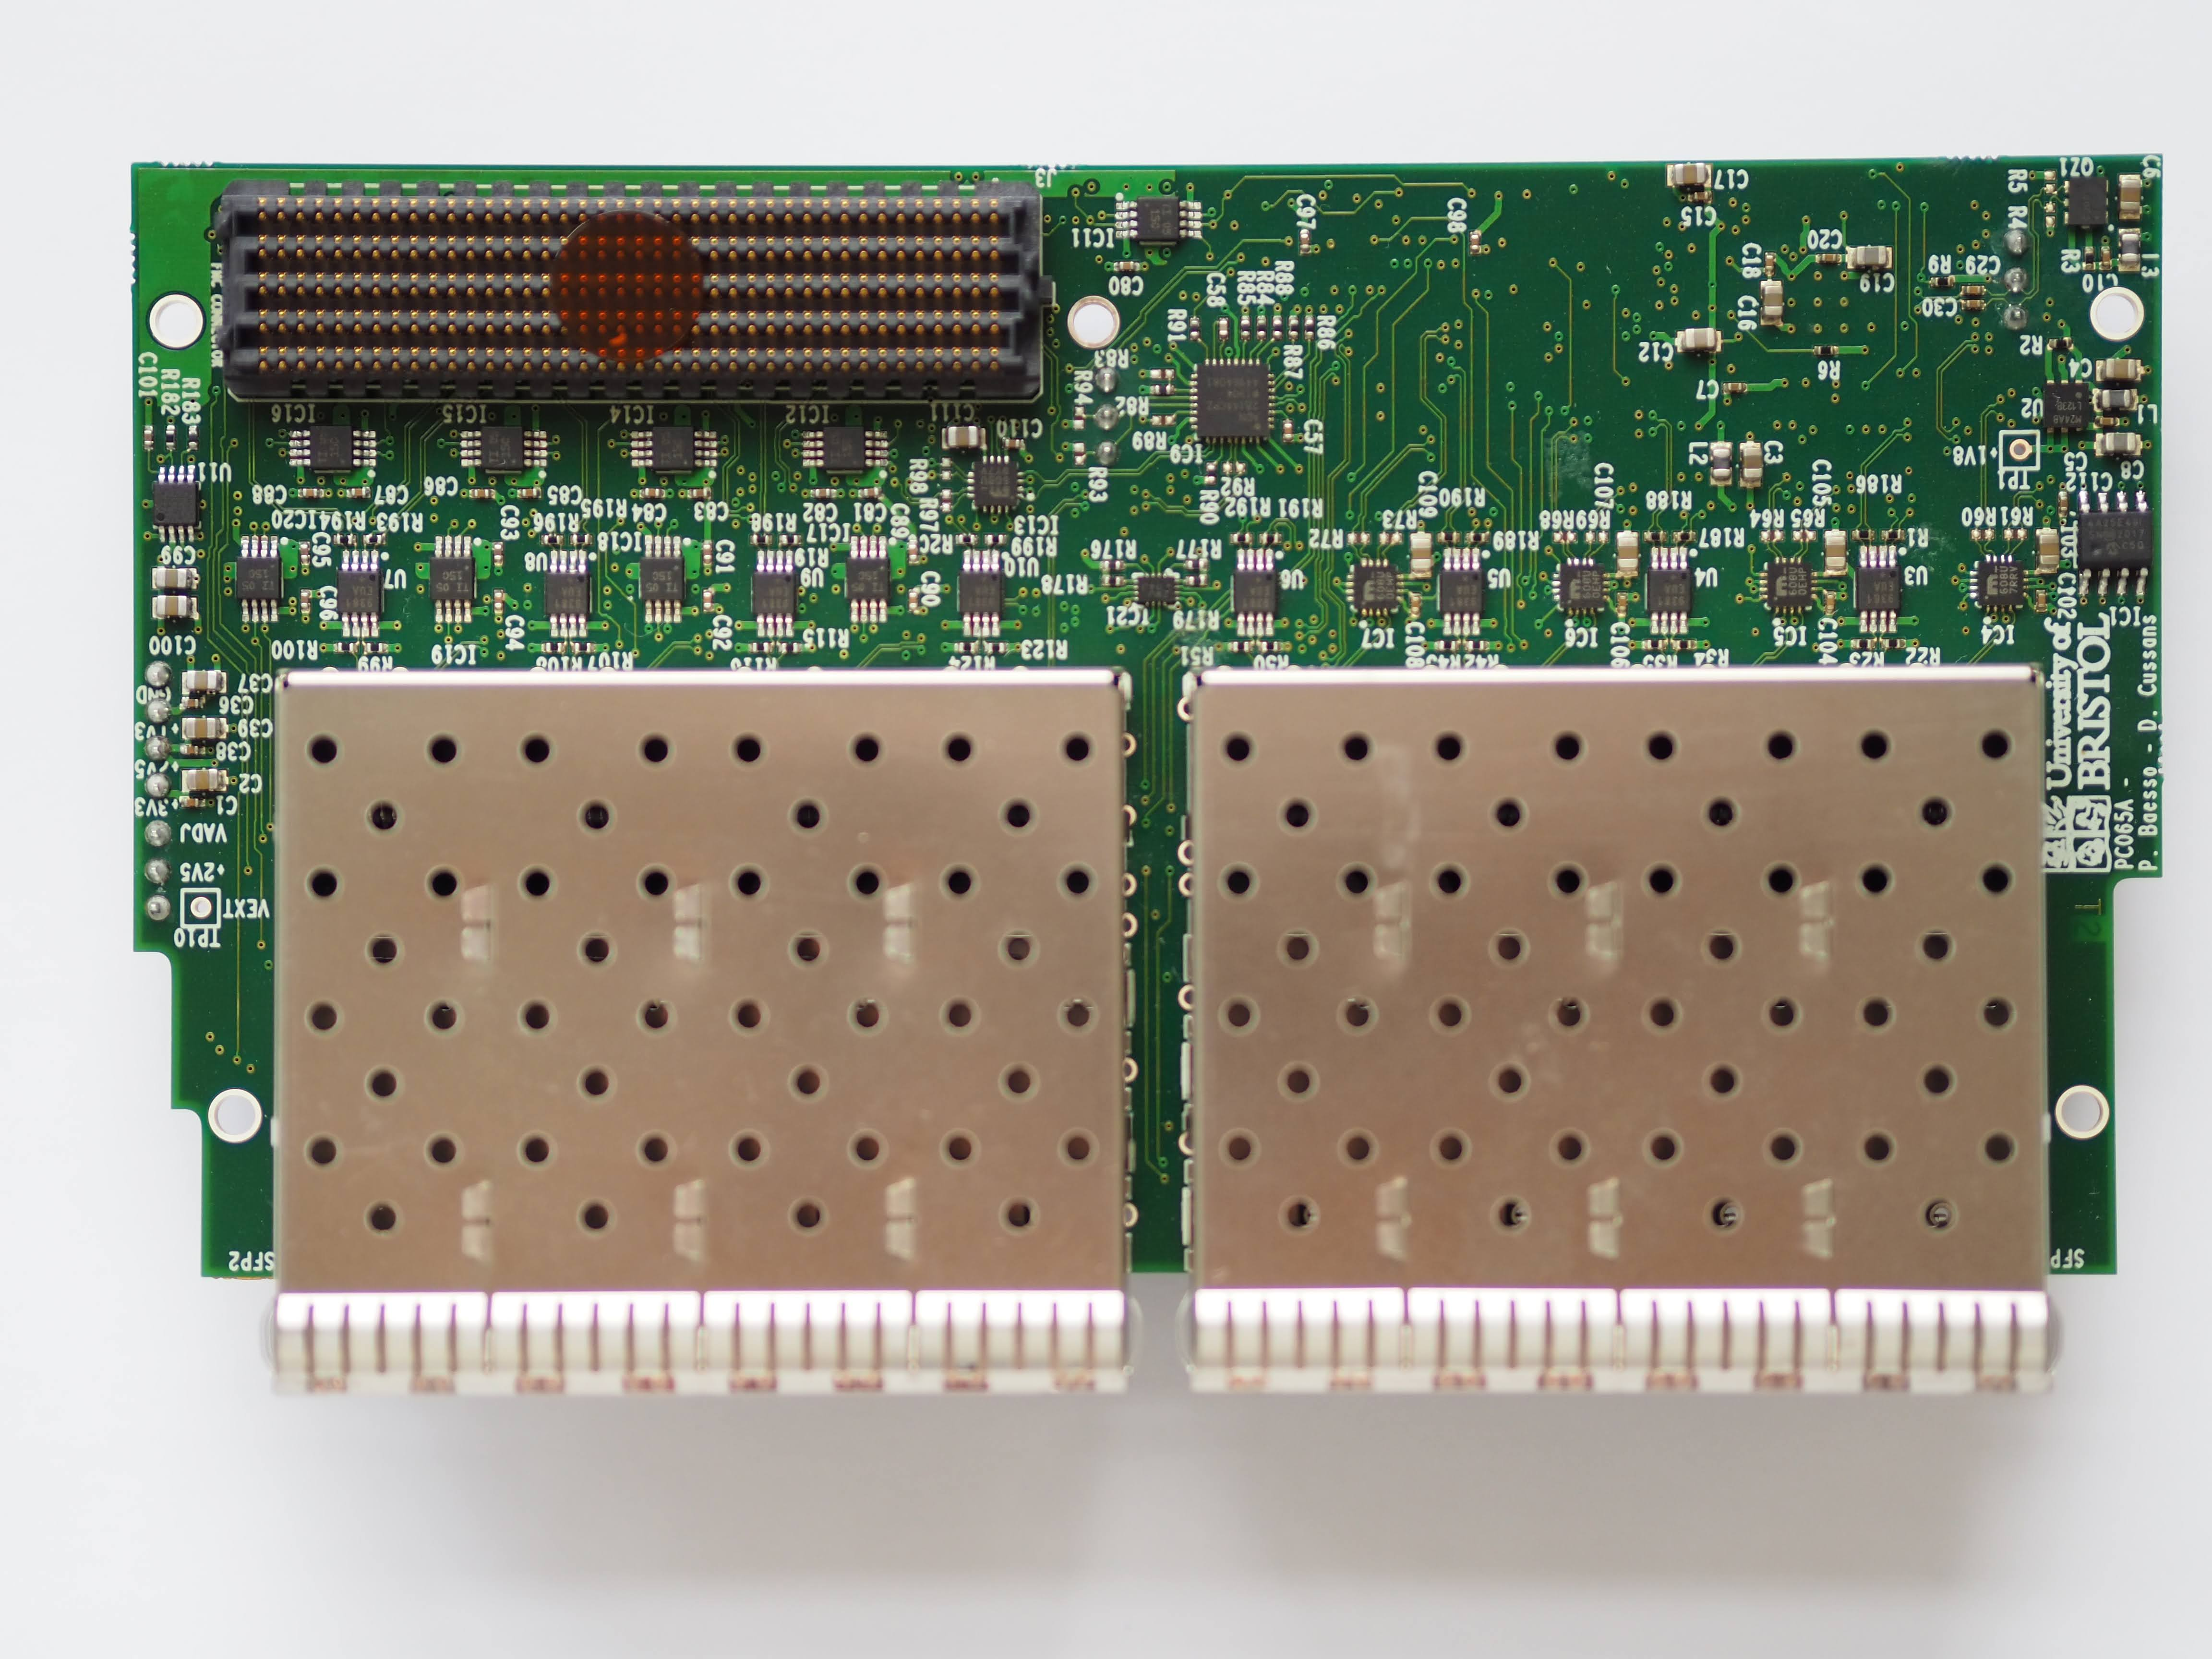
\includegraphics[width=\linewidth]{P7230002.JPG}
  \caption{Photograph of FIB v1.}
  \label{fig:dts-fib-photo}
\end{figure}

\subsubsection{AFC}

The \href{https://ohwr.org/project/afc/wikis/home}{AFC} is an \href{https://ohwr.org}{Open Hardware} design manufactured and supplied by a commercial firm  (\href{https://creotech.pl/}{Creotech}). We are using version-4 of the board with minor modifications to the clocking circuitry. Figure \ref{fig:dts-afc_fib-powering} illustrates the powering arrangements for the AFC/FIB combination. Figure \ref{fig:dts-afc_fib-photo} is a photograph of an AFC with prototype FIB mounted.

\begin{figure}
  \centering
  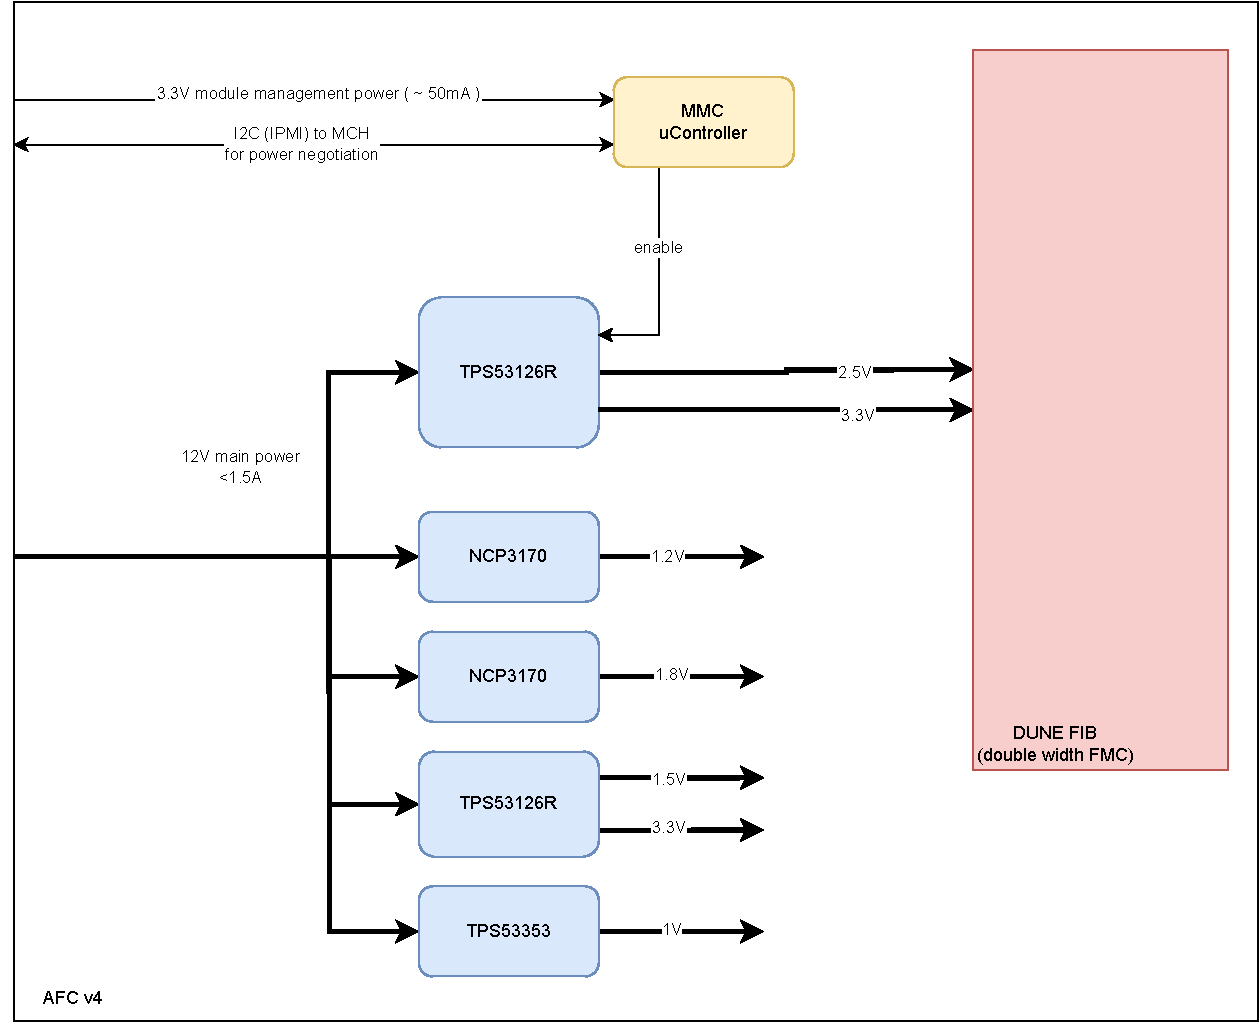
\includegraphics[width=\linewidth]{dts_afc_fib_power_block_diagram_v2-240116.drawio.pdf}
  \caption{Block diagram showing powering of AFC and FIB.}
  \label{fig:dts-afc_fib-powering}
\end{figure}

\begin{figure}
  \centering
  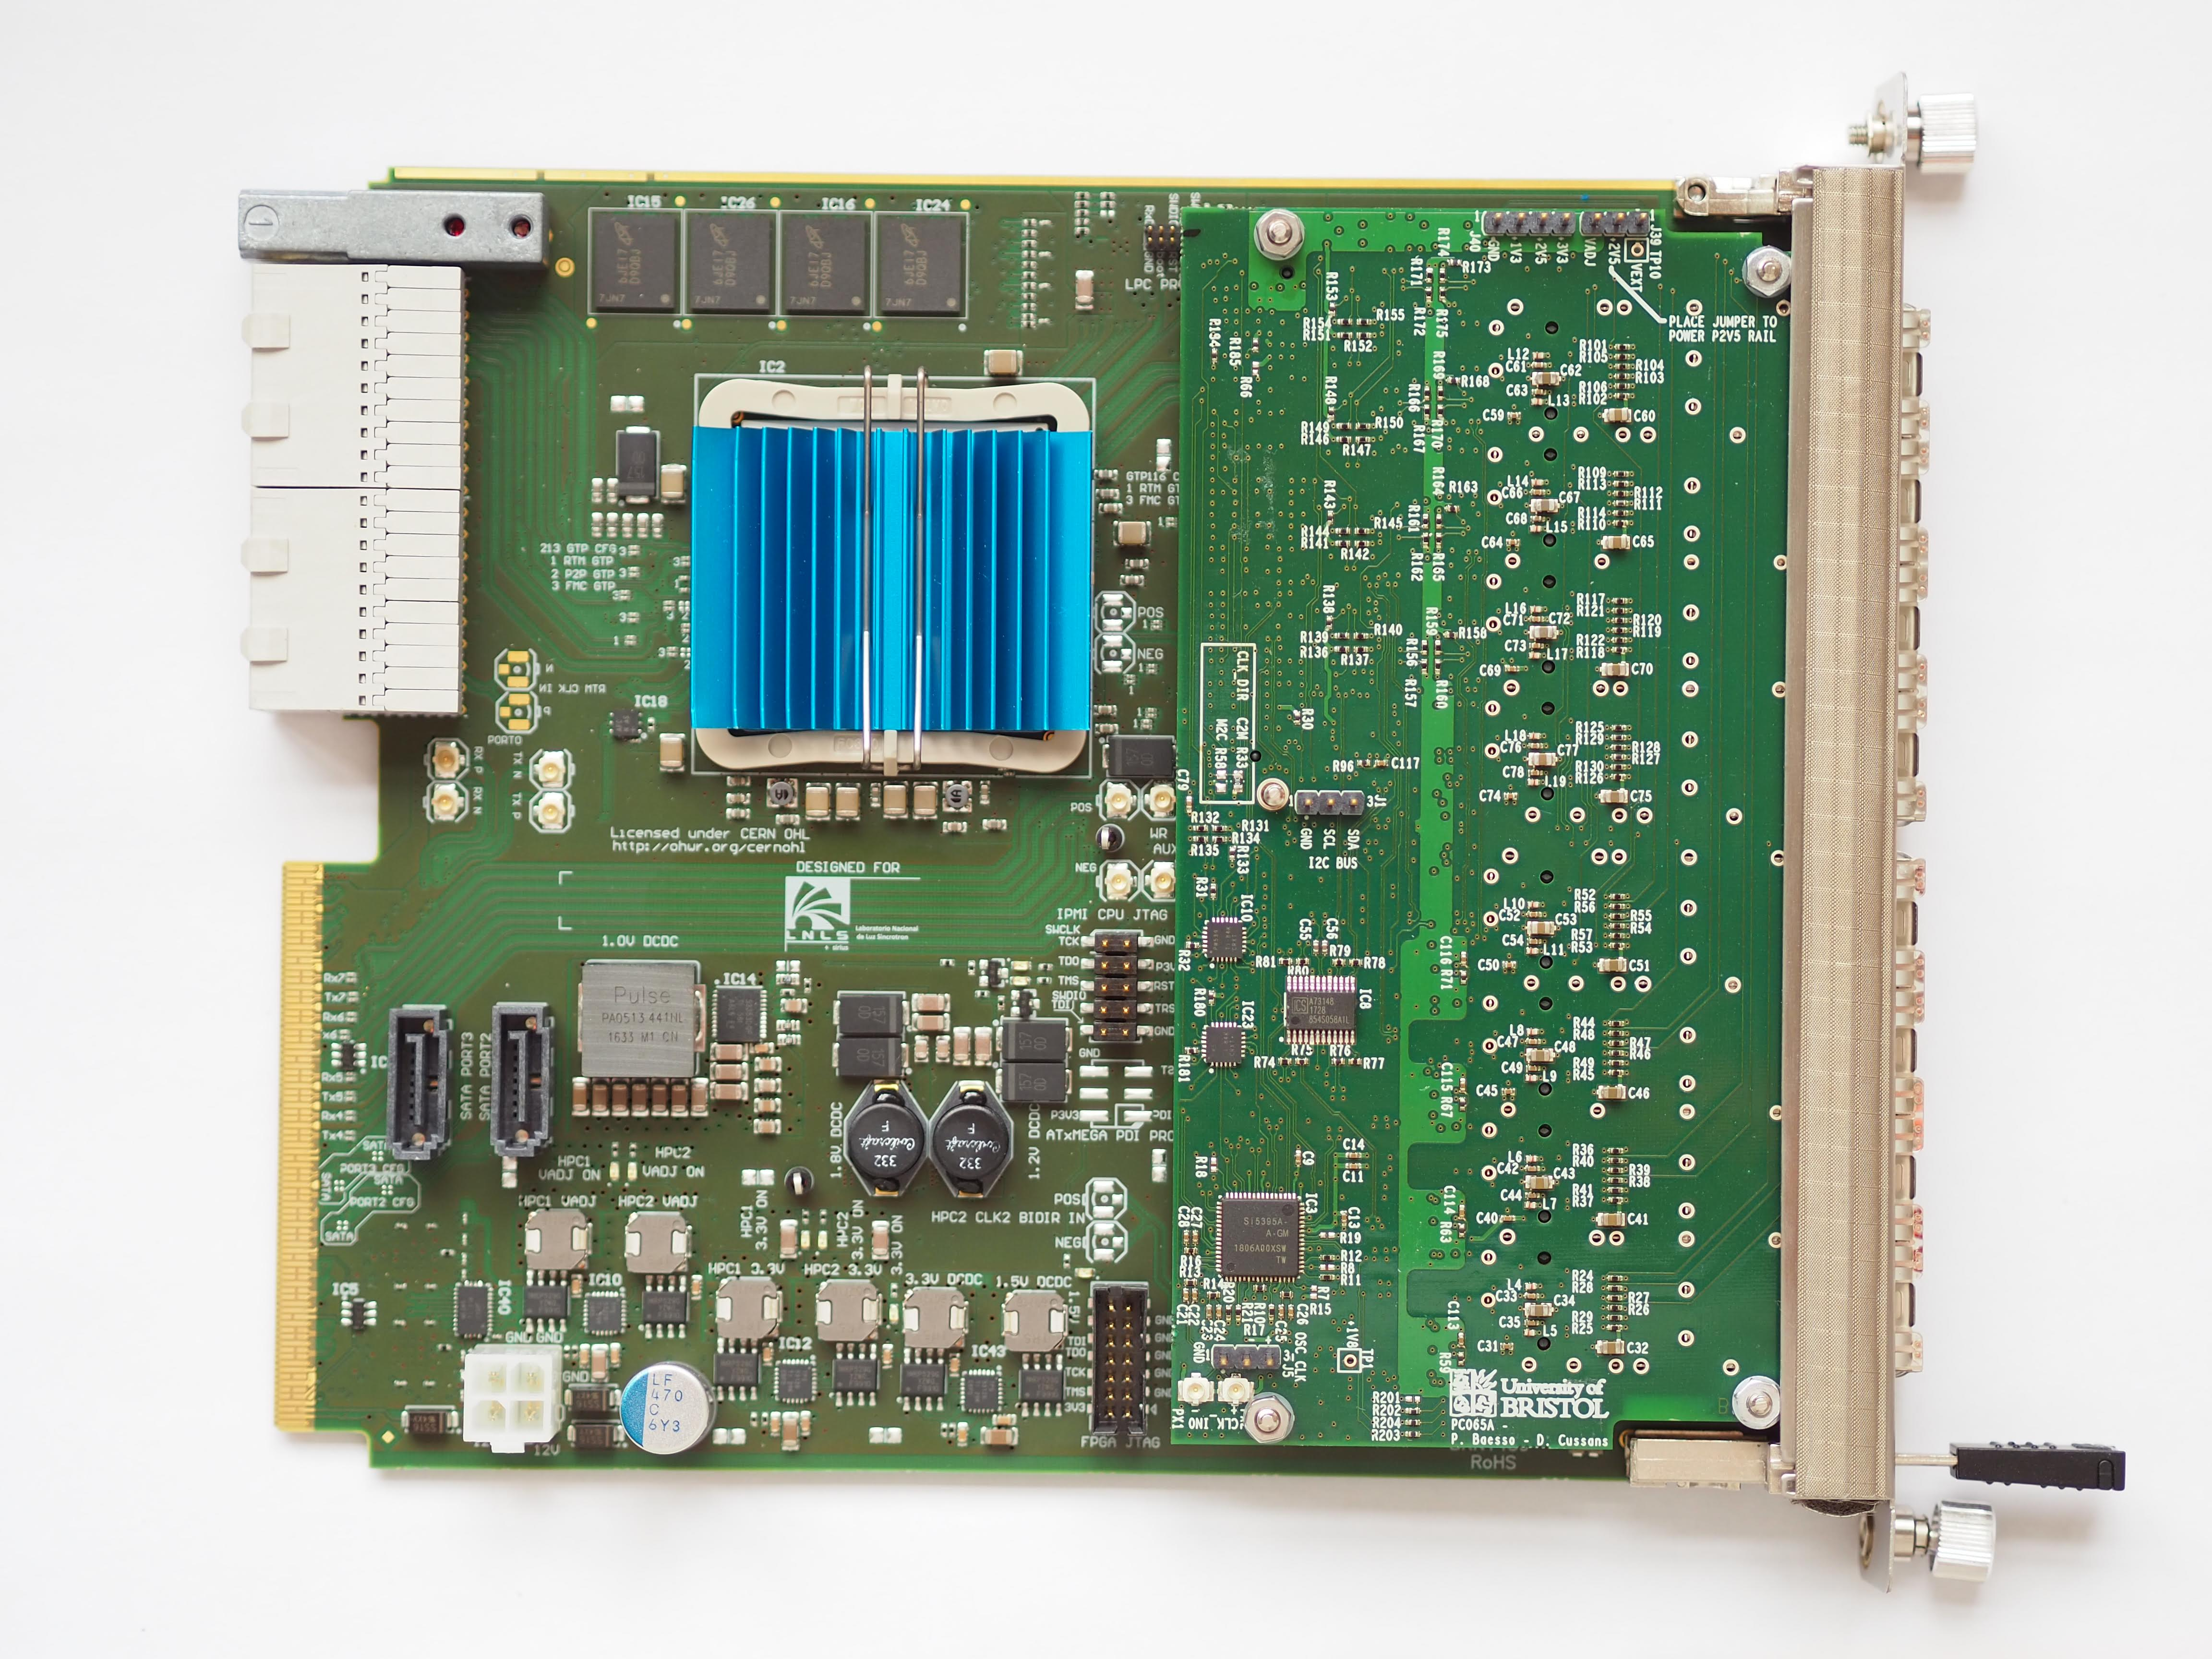
\includegraphics[width=0.8\linewidth]{OI000296.JPG}
  \caption{Photograph of AFC with FIB mounted.}
  \label{fig:dts-afc_fib-photo}
\end{figure}

\section{Electrical Power}

Total electrical power of below ground electrical components is estimated to be 185W $\pm$ 20\% per crate, or 370W per cavern. This is based on a mixture of measurements of prototypes and data sheets of COTS components.

\section{Optical Power}

Each DTS MicroTCA crate will house up to 96 SFP optical transceivers. Each SFP will have a 1000Base-BX interface and a maximum laser power of 2mW at 1490,1550 or 1570nm. Because each individual SFP has an optical output power less than 5mW, and is hence a category 3R laser, no special safety precautions are needed.


%\section*{Acknowledgments}


%\bibliography{sample}

\end{document}